\chapterimage{chapter_head_1.pdf}

\chapter{Bayessche Netze}
\section{Intro}
Ein Bayessches Netz stellt die Wahrscheinlichkeiten von Ereignissen und deren Abhängigkeit (bzw. Unabhängigkeit) zueinander dar.

Bayessche Netze finden immer dort Anwendungsmöglichkeit, wo Logik und Unwissenheit aufeinandertreffen.
Sie dienen der Vereinfachung von komplexen Problemen mit Hilfe weniger stochastischer Regeln.

In der Praxis finden Bayessche Netze beispielsweise in der Spracherkennung, Medizinischen Diagnose, Filtern von Spam, Bildverarbeitung, Analyse von Kaufverhalten und in vielen anderen Gebieten Anwendung.

\begin{figure}[h]
    \centering
    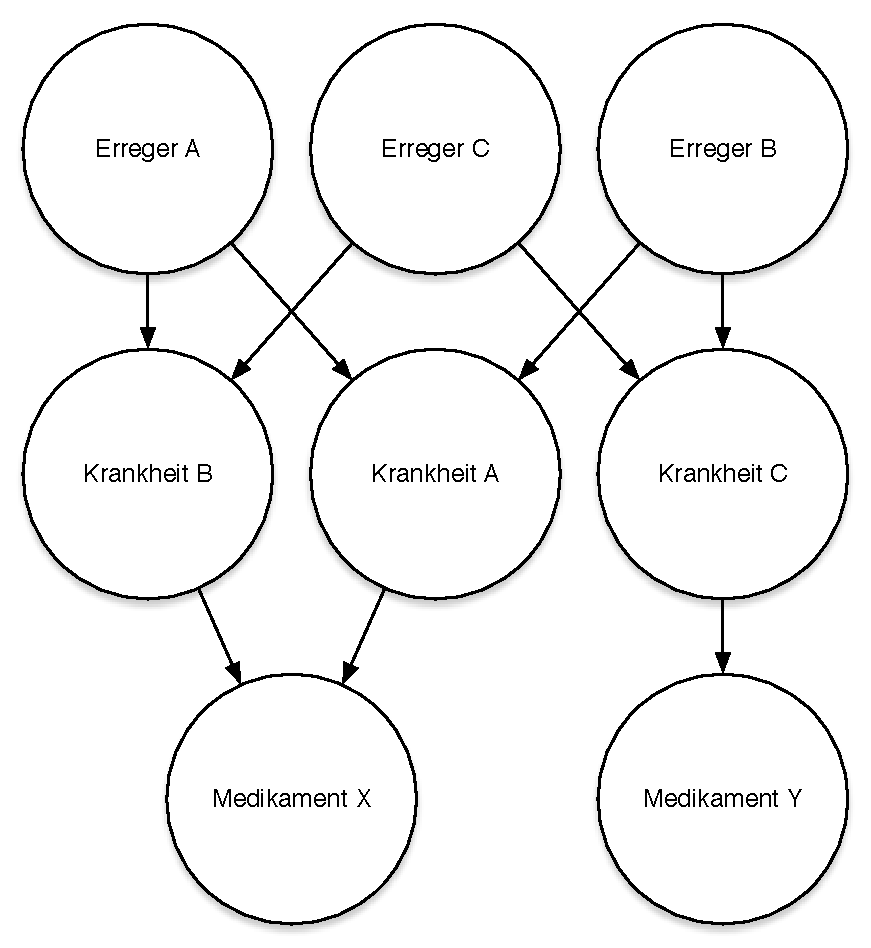
\includegraphics[width=.4\textwidth]{chapters/bayes/bayes_intro.pdf}
    \caption{Beispiel eines Bayesschen Netzes zur Diagnose von Krankheiten (ohne Wahrscheinlichkeiten)}
\end{figure}

\section{Grundlagen der Wahrscheinlichkeitsrechnung}
Einem Ereignis A weisen wir eine Wahrscheinlichkeit p(A) zwischen 0 (tritt nie ein) und 1 (tritt immer ein) zu.

Als marginal probability bezeichnen wir eine Wahrscheinlichkeit p(A), welche keine Abhängigkeiten aufweist.
Beispiel: A=Eine aus einem Skatdeck gezogene Karte ist Kreuz.
p(A)= 1/4 (oder 25\%)

Als joint probability bezeichnen wir Wahrscheinlichkeiten welche nebeneinander auftreten. p(A,B)
Beispiel: A (von oben) und B: Die Karte ist ein Bube

Da A und B voneinander unabhängige Ereignisse sind folgt:
p(A,B) = p(A)*p(B) 1/8*1/4 = 1/32

Sind Ereignisse jedoch nicht unabhängig, so müssen wir die Wahrscheinlichkeit von p(A,B) bereits bestimmt haben.
Möchten wir nun für eine große Anzahl Ereignisse Wahrscheinlichkeiten berechnen, so benötigen wir extrem viele Daten.

\begin{center}
\begin{tabular}{ ccccc } \toprule
Sonne scheint & Werktag & Stau & Rasensprinkler & Tage im Jahr \\ \midrule
F & F & F & F & 4 \\
F & F & F & T & 5 \\
F & F & T & F & 2 \\
F & F & T & T & 1 \\
F & T & F & F & 13 \\
F & T & F & T & 2 \\
F & T & T & F & 66 \\
F & T & T & T & ... \\
T & F & F & F & ... \\
T & F & F & T & \\
T & F & T & F & \\
T & F & T & T & \\
T & T & F & F & \\
T & T & F & T & \\
T & T & T & F & \\
T & T & T & T & Errechenbar \\
\bottomrule
\end{tabular}
\end{center}


Bis auf 1 Errechenbares Ergebnis benötigen wir die direkten Werte aller Kombinationen.
Wir benötigen also Für N Ereignisse $2^N-1$ Datensätze.
Gerade in der Medizin aus dem Anfangsbeispiel gibt es aber oft extrem viele Ereignisse.

Oftmals ist vieles davon aber auch nicht interessant, bzw. ableitbar.
Die Wahrscheinlichkeit, dass die Sonne scheint ist beispielsweise unabhängig davon ob der Tag ein Werktag ist.

Um die benötigten Datensätze möglichst gering zu halten betrachtet man bedingte Wahrscheinlichkeiten (conditional probability).

\section{Bedingte Wahrscheinlichkeit}
Bedingte Wahrscheinlichkeiten beruhen auf Annahmen.
Man nimmt etwa an, dass Die Sonne keinen Einfluss auf die Frage hat, ob es nun ein Werktag ist, sehr wohl jedoch auf die Frage, ob der Sprinkler angeschaltet ist.
Gehen wir weiterhin davon aus, dass an sonnigen Tagen mehr Staus zustande kommen, da z.B. Fahrer geblendet werden.
Zudem gehen wir davon aus, dass Werktags mehr Staus auftreten.
Fügen wir zudem noch das Verpassen des Essens hinzu, welches lediglich vom Stau abhängt.

\begin{figure}[h]
    \centering
    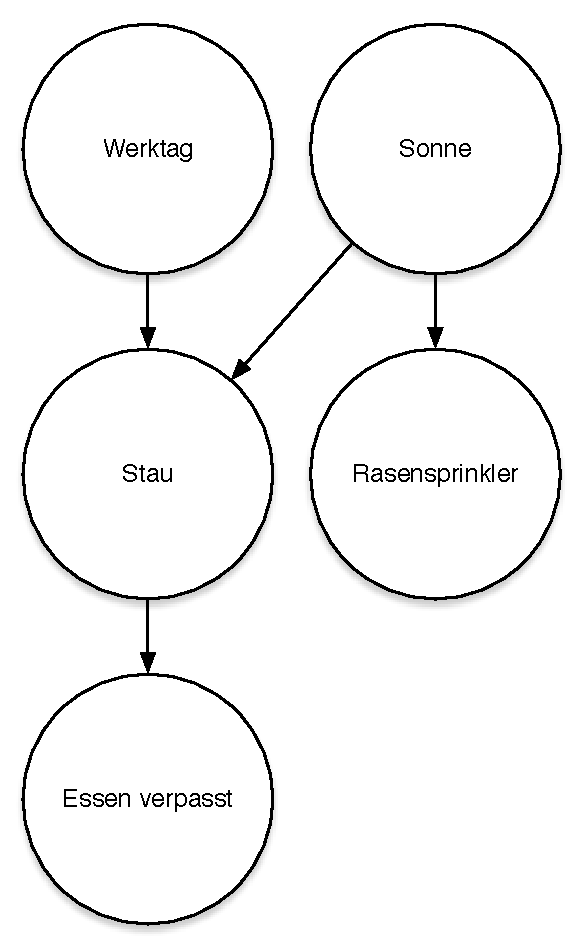
\includegraphics[width=.2\textwidth]{chapters/bayes/bayes_example.pdf}
\end{figure}

Unsere benötigten Datensätze mit fiktivem Inhalt:\\
$p(Sonne) = 0.8$\\
$p(Werktag)= 0,7$\\
$p(Rasensprinkler | Sonne) = 0.95$\\
$p(Rasensprinkler | !Sonne) = 0.20$\\
$p(Stau | Sonne,Werktag) = 0.8$\\
$p(Stau | !Sonne, Werktag) = 0.75$\\
$p(Stau | Sonne, !Werktag) = 0.15$\\
$p(Stau | !Sonne, !Werktag) = 0.05$\\
$p(Essen verpasst | Stau) = 0.5$\\
$p(Essen verpasst | !Stau) = 0.05$\\

Von 31 Datensätzen in einer Tabelle mit joint probabilities haben wir nun nur noch 10 benötigt Wahrscheinlichkeiten und können alle anderen nun Problemlos errechnen. (Beispiel folgt)

Um bedingte Wahrscheinlichkeiten effektiv nutzen zu können benötigen wir einige Definitionen:
\begin{equation*}
p(A,B) = p (A | B) * p (B)
\end{equation*}
Daraus folgt direkt:
\begin{equation*}
p(A,B,C) = p(A | B,C)* p(B,C) = p(A | B,C) * p(B | C) *p(C)
\end{equation*}
Dies lässt sich für N Ereignisse wie folgt darstellen (Chain Rule):
\begin{equation*}
    P\left(\bigcap_{k=1}^n A_k\right)  = \prod_{k=1}^n  \mathrm P\left(A_k \,\Bigg|\, \bigcap_{j=1}^{k-1} A_j\right)
\end{equation*}
Zudem bezeichnen wir A als von B unabhängig, wenn gilt:
\begin{equation*}
p(A | B) = p(A)
\end{equation*}
und A als von B unabhängig unter der Prämisse C, wenn gilt:
\begin{equation*}
p(A | C)* p(B | C) = p(A,C | B)
\end{equation*}

Mit Hilfe der Chain-Rule können wir nun für das Beispiel von oben jede mögliche joint probability ausrechnen.

Beispiel:
p(Essen verpasst,Stau,Werktag,Rasensprinkler,Sonne)
nach Anwendung der Chain Rule haben wir:
p(Essen verpasst | Stau,Werktag,Rasensprinkler,Sonne) \\ *p(Stau | Werktag , Rasensprinkler, Sonne) \\ *p(Werktag | Rasensprinkler, Sonne)
\\ *p( Rasensprikler | Sonne)
\\ *p(Sonne)

Wichtig ist hier den Aufbau des ersten Ausdrucks entlang der Abhängigkeiten zu formulieren. Die Reihenfolge der Ereignisse für die joint probabilty muss also eine umgedrehte topologische Anordnung unseres Graphen darstellen bzw. ein Ereignis A kann nicht vor einem Ereignis B stehen, wenn B abhängig von A ist.

Nach dem kürzen der Unabhängigkeiten erhalten wir:
p(Essen verpasst | Stau ) * p( Stau | Werktag, Sonne) * p( Werktag) * p( Rasensprinkler | Sonne) * p(Sonne)

Man nennt dies auch die Faktorisierung.

Die gesuchten Wahrscheinlichkeiten kennen wir bereits und können sie Einsetzen:
0,5*0,8*0,7*0,95*0,8 = 0,218.

Es ist also durch simples Einsetzen unserer 10 Werte möglich sämtliche 31 Werte für die joint probability Tabelle zu berechnen.
Gleichzeitig sind Lösungen für relevante Fragen zur bedingten Wahrscheinlichkeit, welche nicht alle Ereignisse umfassen, mit geringem Aufwand zu lösen.


In der Regel sind jedoch nicht alle Angaben bekannt.
Nehmen wir nun an, dass wir als hart arbeitender Mensch an einem Nicht-Werktag zur Arbeit fahren und es sonnig ist.
Wir möchten nun wissen, wie Wahrscheinlich es ist, dass man es abends bei der Rückfahrt rechtzeitig zum Essen schafft.
Wir suchen also p(!Essen verpasst | !Werktag, Sonne)

Dazu berechnen wir:
p(!Essen verpasst | Stau )*p(Stau |Sonne, Werktag) + p(!Essen verpasst | !Stau)*p(!Stau | Sonne, Werktag)

Die passenden Werte kennen wir entweder oder können sie direkt ableiten.
p(Essen verpasst | Stau) = 0.5
p(Essen verpasst | !Stau) = 0.05
p(Stau | Sonne, !Werktag) = 0.15

0,5*0,15+0,95*0.85 = 0,8825 bzw. die Wahrscheinlichkeit am Wochenende pünktlich zum Essen zu kommen ist 88\%.

Was jedoch, wenn ich in die andere Richtung rechnen möchte?
Beispiel: Der Lebensgefährte kommt pünktlich zum Essen und ich möchte Wissen, wie wahrscheinlich es ist, dass er im Stau gesteckt hat.

Wir kennen bereits die Formel:\\
p(A,B) = p (A | B) * p(B) offensichtlich gilt auch\\
p(B,A) = p (B | A) * p(A) wir folgern daraus:\\
p(A | B) = p(A,B) / P(B) = p(B,A) / P(B) = p(B | A) * p(A)/p(B)

Wir wissen also:
p(Stau | !Essen verpasst) = p(!Essen verpasst | Stau ) *P(Stau)/p(! Essen verpasst)

p(!Essen verpasst | Stau) =0,5\\
p(Stau) =\\
p(Stau | Sonne, Werktag)*p(Sonne)*p(Werktag) + \\ p(Stau | Sonne, !Werktag)*p(Sonne)*p(!Werktag)+ \\ p(Stau | !Sonne, Werktag)*p(!Sonne)*p(Werktag) + \\ p(Stau | !Sonne, !Werktag)*p(!Sonne)*p(!Werktag)\\ =0,382

p(!Essen verpasst) =\\
p(!Essen verpasst | Stau)*p(Stau)\\ + p(!Essen verpasst | !Stau)*p(!Stau)\\ =0.7781

=> p(Stau | !Essen verpasst)=0,5*0,382/0,7781 = 0,2454...

Ist die Person also pünktlich, so gab es mit einer Wahrscheinlichkeit von ~75\% keinen Stau.

An dieser Stelle ist anzufügen, dass das ganze Problem auch so hätte modelliert werden können, dass die Pünktlichkeit beim Essen ebenfalls vom Werktag abhängig ist, dann jedoch wäre die Abhängigkeit zum Stau zu hinterfragen, wenn es denn keinen Werktag gibt.
Es gibt also durchaus komplexere Problemstellungen, die wir mit unseren einfachen Methoden nicht so einfach behandeln können und eventuell verschiedene Modelle für Abhängigkeiten die je nach der Menge der Daten möglicherweise nicht optimal sind.

Diese neue Methode hilft uns vor allen Dingen damit mit einem einzelnen Modell gleichzeitig z.B. Krankheiten und Symptome in beide Richtungen zu bestimmen. Ohne große Umstände kann eine Krankheit aus Symptomen bestimmt werden und direkt von der Wahrscheinlichkeit der Krankheit kann die Wahrscheinlichkeit für weitere Symptome berechnet werden.

\section{Graphische Darstellung}
\begin{figure}[h]
    \centering
    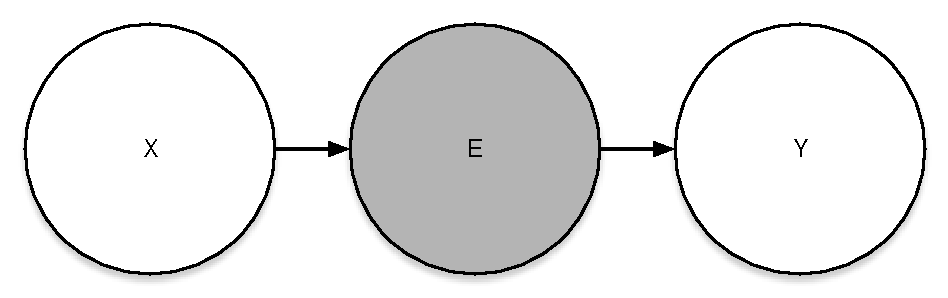
\includegraphics[width=.2\textwidth]{chapters/bayes/bayes_net_1.pdf}
\end{figure}
\begin{figure}[h]
    \centering
    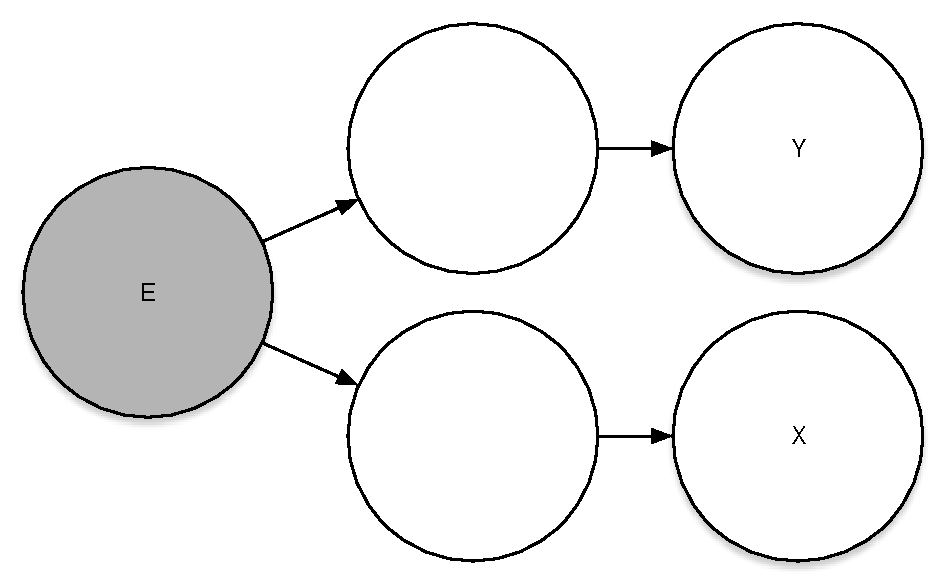
\includegraphics[width=.2\textwidth]{chapters/bayes/bayes_net_2.pdf}
\end{figure}
\begin{figure}[h]
    \centering
    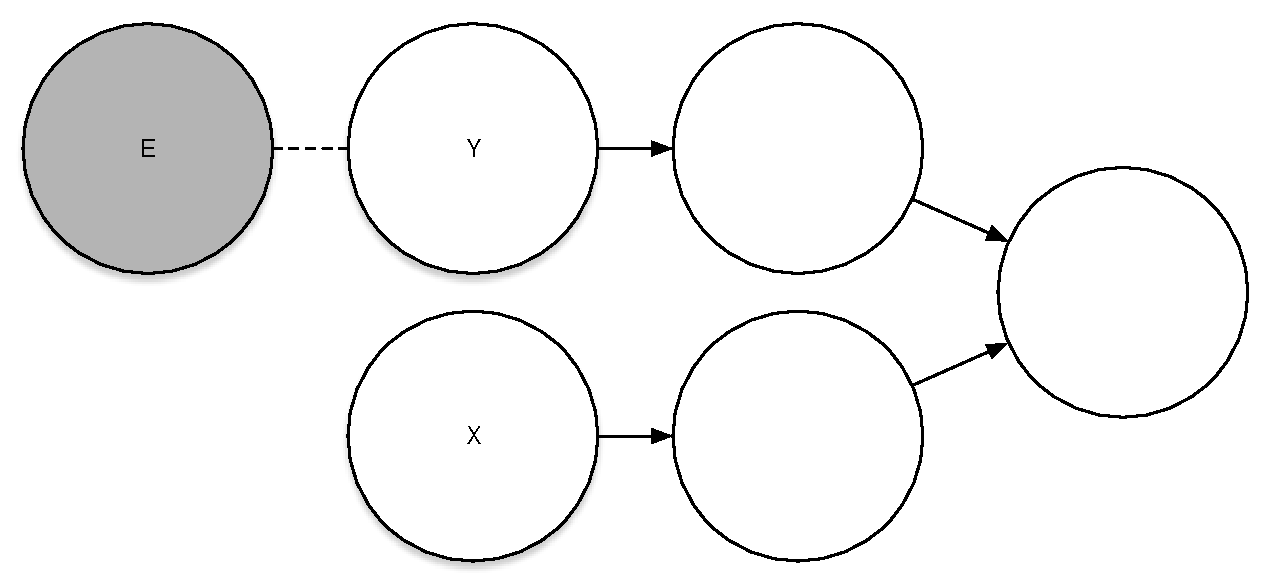
\includegraphics[width=.2\textwidth]{chapters/bayes/bayes_net_3.pdf}
\end{figure}
\begin{figure}[h]
    \centering
    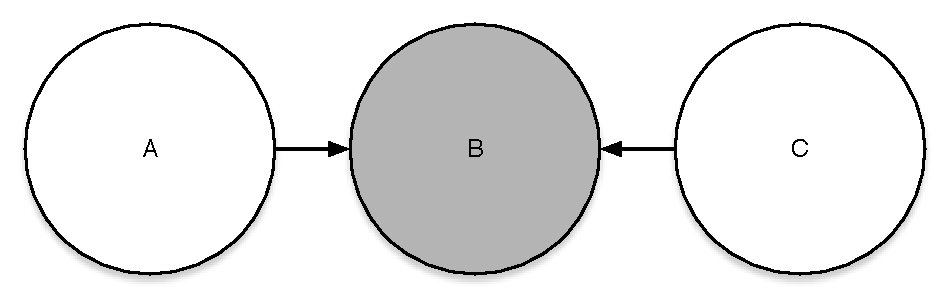
\includegraphics[width=.2\textwidth]{chapters/bayes/bayes_net_4.pdf}
\end{figure}

Wir nennen Zwei Ereignisse X und Y bedingt unabhängig gegeben E, wenn im Graphen kein Weg von X zu Y existiert, welcher nicht E nicht beinhaltet.
Dies wir auch d-seperation genannt.
Wir schreiben hierfür
$X \perp Y | E$
Ausgehend vom vorherigen Beispiel heißt das, dass das Verpassen des Essens zwar vom Werktag abhängt, jedoch wenn bekannt ist, ob es einen Stau gab, diese Abhängigkeit aufgehoben wird.
Für 3 verknüpfte Ereignisse gibt es die Folgenden Möglichkeiten:
\begin{enumerate}[label=(\alph*)]
\item $A \rightarrow B \rightarrow C$ impliziert $A \perp C | B$
\item $A \leftarrow B \leftarrow C$ impliziert $A \perp C | B$
\item $A \leftarrow B \rightarrow C$ impliziert $A \perp C | B$
\item $A \rightarrow B \leftarrow C$ impliziert $A \perp C$
\end{enumerate}
Das Beispiel (d) beschreibt hierbei eine sogenannte V-Struktur.

Betrachten wir hierzu außerdem die Verschiedenen Faktorisierungen:
\begin{enumerate}[label=(\alph*)]
\item p(A,B,C)=p(C| B)*p(B|A)*p(A)
\item p(A,B,C)=p(A| B)*p(B|C)*p(C)
\item p(A,B,C)=p(A| B)*p(C|B)*p(B)
\item p(A,B,C)=p(B| A,C)*p(A)*p(C)
\end{enumerate}

\section{IC-Algorithmus}
Der IC Algorithmus ist eine Möglichkeit aus gegebenen Unabhängigkeiten ein Bayessches Netz zu erstellen.
\begin{enumerate}
\item Konstruiere einen ungerichteten Graphen gibt füge jede mögliche Kante (X,Y) für die es keine (bedingte) Abhängigkeit $X \perp Y | E$ bzw. $X \perp Y$ gibt in den Graphen ein.
\item Gilt für zwei Nachbarn X,Y von einem Knoten E die bedingte Unabhängigkeit $X \perp Y | E$, dann füge die Kanten (X,E) und (Y,E) hinzu. (V-Struktur)
\item Orientiere die Verbleibenden Kanten beliebig, aber ohne neue v-Strukturen entstehen zu lassen.
\end{enumerate}

\section{Quellen}
\begin{itemize}
\item Open Course „Artifical Intelligence“ am MIT
\item https://upload.wikimedia.org/math/b/5/a/b5a87dba9ec79dd6a93628c85fab ca97.png
\item http://www.informatik.uni-bremen.de/tdki/lehre/ss12/bayes/Intro.pdf
\item http://www.fil.ion.ucl.ac.uk/~wpenny/bdb/bayes.pdf
\item Bayesian Artificial Intelligence, Second Edition
\end{itemize}
